\documentclass{beamer}
\usepackage[latin1]{inputenc}
\usepackage[ngerman]{babel}
\usepackage{graphicx}
\usepackage{graphics}
\usepackage{enumerate}
\usepackage{amsmath}
\usepackage{amsfonts}
\usepackage{amssymb}
\usepackage{beamerthemesplit}

\setbeamertemplate{navigation symbols}{}
\setbeamertemplate{items}[ball]
\setbeamertemplate{blocks}[rounded][shadow=true]

%%%%%%%%%%%%%%%%%%%%%%%%%%%%%%%%%%%%%%%%%%%%%%%%
%%% set theme %%%%%%%%%%%%%%%%%%%%%%%%%%%%%%%%%%
%%%%%%%%%%%%%%%%%%%%%%%%%%%%%%%%%%%%%%%%%%%%%%%%

%\usetheme{Rochester}
%\usetheme{Szeged}
%\usetheme{Dresden}
%\usetheme{Berlin}
\usetheme{Ilmenau}
%\usetheme{Frankfurt}
%\usetheme{Warsaw}
%\usecolortheme{orchid}

%%%%%%%%%%%%%%%%%%%%%%%%%%%%%%%%%%%%%%%%%%%%%%%%
%%% setup document %%%%%%%%%%%%%%%%%%%%%%%%%%%%%
%%%%%%%%%%%%%%%%%%%%%%%%%%%%%%%%%%%%%%%%%%%%%%%%

\title{Discriminative Classifier Parts}
\author{Christoph Bichler and Robert Viehauser}
\date{24. January 2013}


%%%%%%%%%%%%%%%%%%%%%%%%%%%%%%%%%%%%%%%%%%%%%%%%
%%% create frames %%%%%%%%%%%%%%%%%%%%%%%%%%%%%%
%%%%%%%%%%%%%%%%%%%%%%%%%%%%%%%%%%%%%%%%%%%%%%%%

\begin{document}
\frame{\titlepage
\begin{center}
\centering
Supervisor: Samuel Schulter \\ \vspace{5mm}
Ausgew�hlte Kapitel Computer Vision
\end{center}
} % creates titlepage

%%%%%%%%%%%%%%%%%%%%%%%%%%%%%%%%%%%%%%%%%%%%%%%%%%%%%%%%%%%%%%%%%%%%%%%%%%%%%%%%%%%%%%%%%%%%%%%%%%%%%%%%%
\section{Introduction}
\subsection{}
%%%%%%%%%%%%%%%%%%%%%%%%%%%%%%%%%%%%%%%%%%%%%%%%%%%%%%%%%%%%%%%%%%%%%%%%%%%%%%%%%%%%%%%%%%%%%%%%%%%%%%%%%

\begin{frame}
\frametitle{Discriminative Patches}
\begin{block}{What are \underline{discriminative} patches?}
\begin{figure}
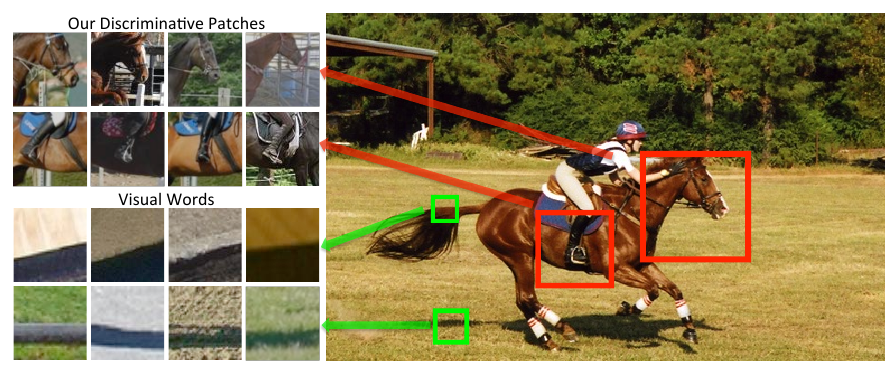
\includegraphics[scale = 0.4]{pics/1_the_idea.png}
\end{figure}
\end{block}

\begin{block}{Paper}
 Saurabh Singh et al: Unsupervised Discovery of Mid-level Discriminative Patches, ECCV 2012
\end{block}


\end{frame}

\begin{frame}
\frametitle{Discriminative Patches}
We want patches that represents the essence of the image, not just its gradients!
\begin{block}{Required properties}
\begin{itemize}
\item Representative
\item Discriminative enough from the rest of the world
\end{itemize}
\end{block}

\end{frame}


\begin{frame}
\frametitle{Motivation}

\begin{block}{Opens doors for further research}
\begin{itemize}
\item More complex classification
\item Scene understanding
\end{itemize}
\end{block}

\begin{block}<2->{Example}
\begin{itemize}
\item What makes Paris look like Paris? \footnote{C.Doersch, et al. What Makes Paris Look like Paris? (SIGGRAPH 2012)}
\end{itemize}
\end{block}

\end{frame}


\begin{frame}
\frametitle{Motivation - What makes Paris look like Paris?}
\begin{block}{Give it a try!}
$\begin{array}{cc}
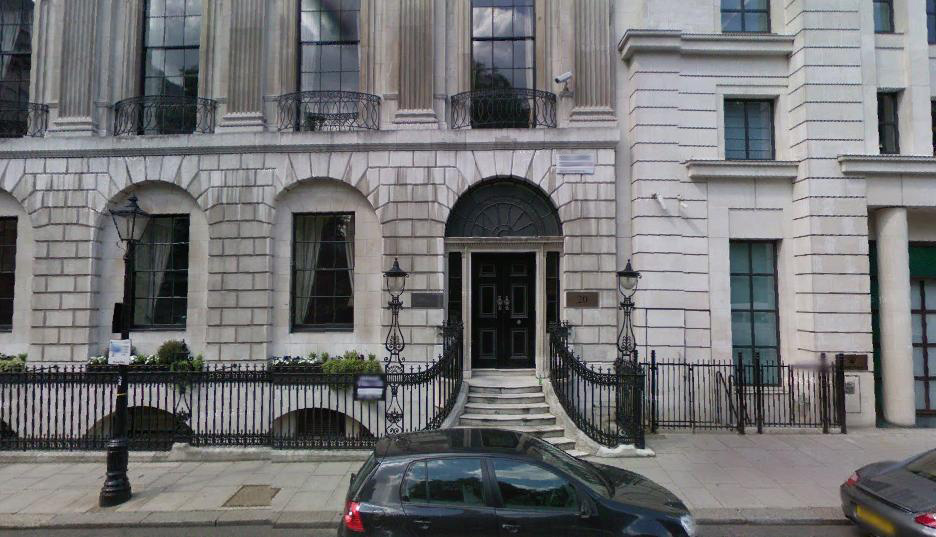
\includegraphics[scale = 0.15]{pics/not_paris.jpg} &
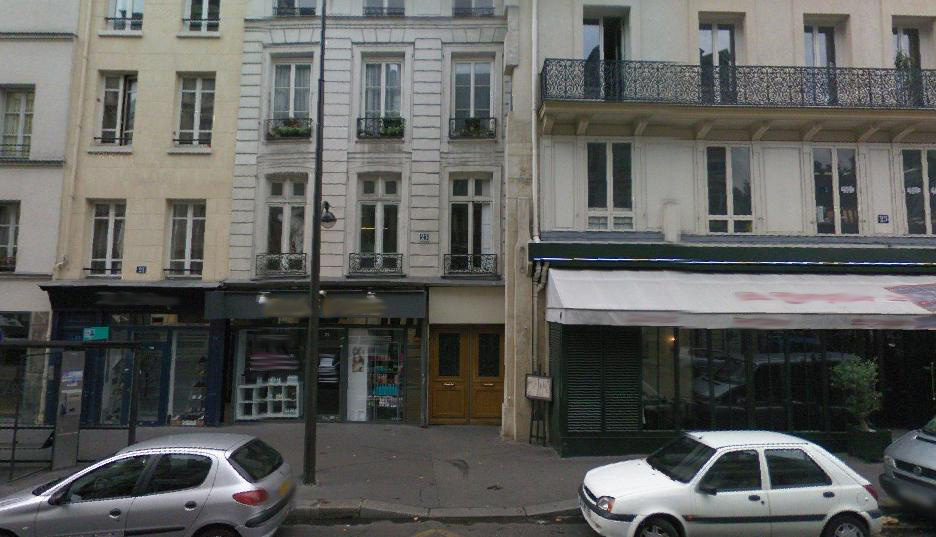
\includegraphics[scale = 0.15]{pics/paris.jpg}
\end{array}$
\end{block}

\begin{block}<2->{Guessed right?}
\begin{itemize}
\item Image 1: Non Paris (London),  Image 2: Paris
\end{itemize}
\end{block}

\end{frame}


\section{Method}
\subsection{}
\begin{frame}
\frametitle{Idea}

Unsupervised learning of "discriminativeness"\\
(without any evidence of humans)

\begin{block}<2->{Basic Process}
\begin{itemize}
\item<2-> Learning patches from the interesting set (discovery set $\mathcal{D}$)
\\against the rest of the world (large "natural world set" $\mathcal{N}$)
\item<2-> Shared feature space: HOG Descriptor
\item<2-> Learning Methods: k-Means + Support Vector Machine
\item<2-> Determining clusters of the same "visual concept"
\item<2-> Choosing the top members of the "best" few Clusters
\end{itemize}
\end{block}

\end{frame}


\begin{frame}
\frametitle{The Algorithm}

\begin{block}{Pseudocode}
\begin{figure}
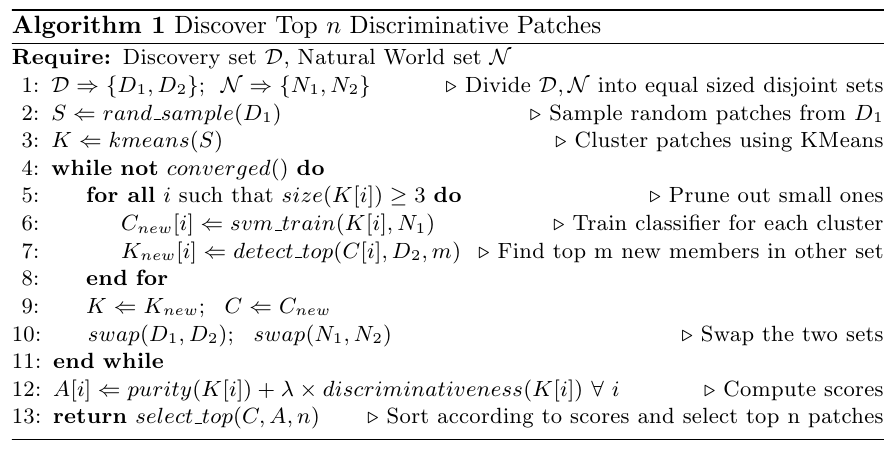
\includegraphics[width= 0.9\textwidth]{pics/algorithm.png}\\
\tiny{Source: Saurabh Singh et al.: Unsupervised Discovery of Mid-level Discriminative Patches, ECCV 2012}
\end{figure}
\end{block}

\end{frame}


\begin{frame}
\frametitle{The Algorithm}

\begin{block}{Drawbacks of unsupervised method}
\begin{itemize}
\item Many patches are needed in the discovery set $\mathcal{D}$
\item Even more in the natural world set $\mathcal{N}$ (tens of millions?)
\item Very memory and computation time consuming!
\end{itemize}
\end{block}

\begin{block}<2->{Problems (especially we had)}
\begin{itemize}
\item Running out of memory
\item Very long runtime ($\sim 7\textendash 8h$ per test)
\item Disappointing results due to a too small world set and mismatched parameters
\item Less technical details known (source code not ready yet)
\end{itemize}
\end{block}

\end{frame}



\section{Experiments}
\subsection{Pascal VOC 2007}
\begin{frame}
\frametitle{Busses}
\begin{figure}
\includegraphics[height = 0.85\textheight]<2->{pics/bus_iter1.png}
\end{figure}
\end{frame}

\begin{frame}
\frametitle{Busses}
\begin{figure}
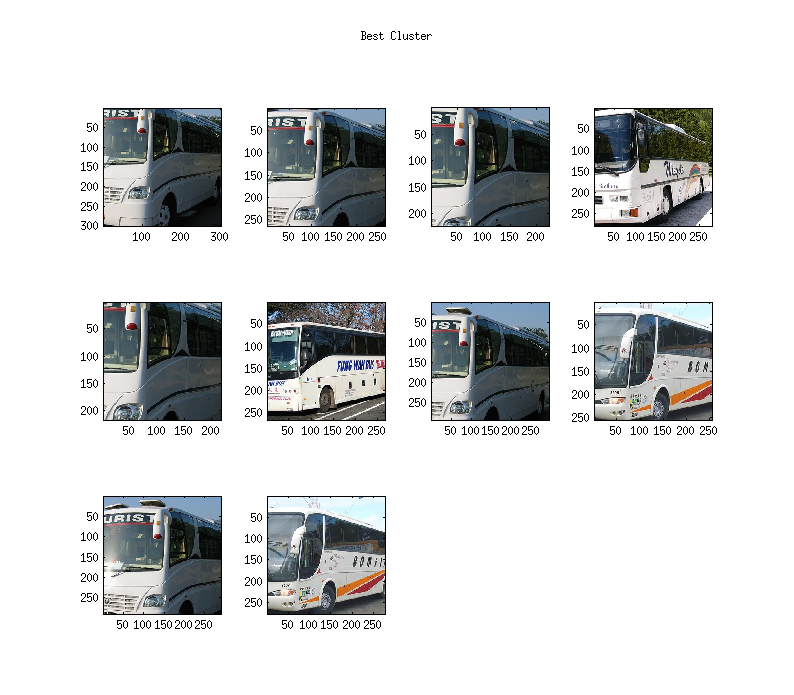
\includegraphics[height = 0.8\textheight]{pics/bus_best1.png}
\end{figure}
\end{frame}

\begin{frame}
\frametitle{Busses 2}
\begin{figure}
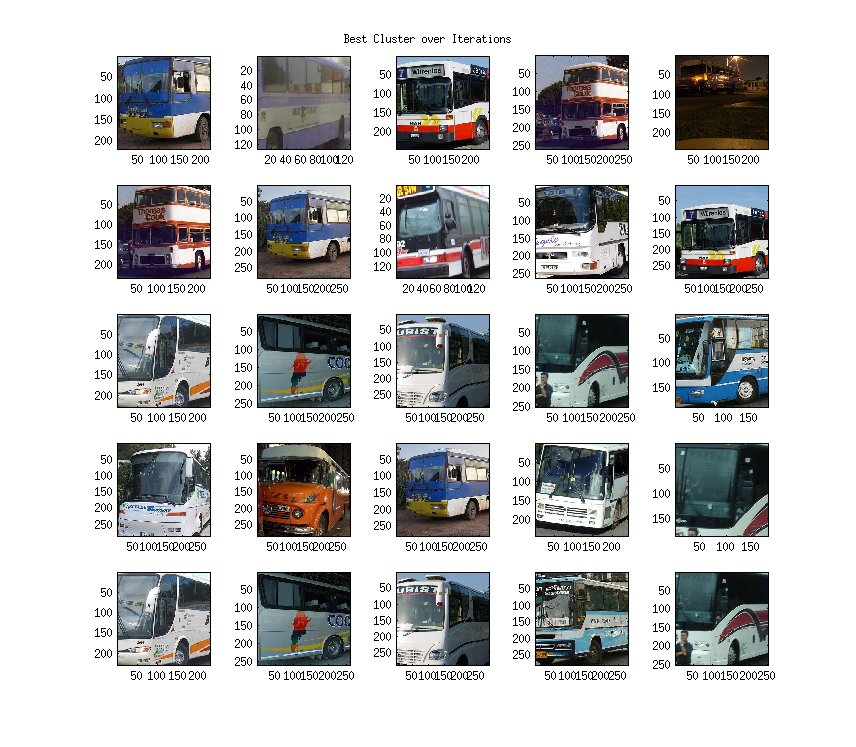
\includegraphics[height = 0.85\textheight]{pics/bus_iter2.png}
\end{figure}
\end{frame}

\begin{frame}
\frametitle{Busses 2}
\begin{figure}
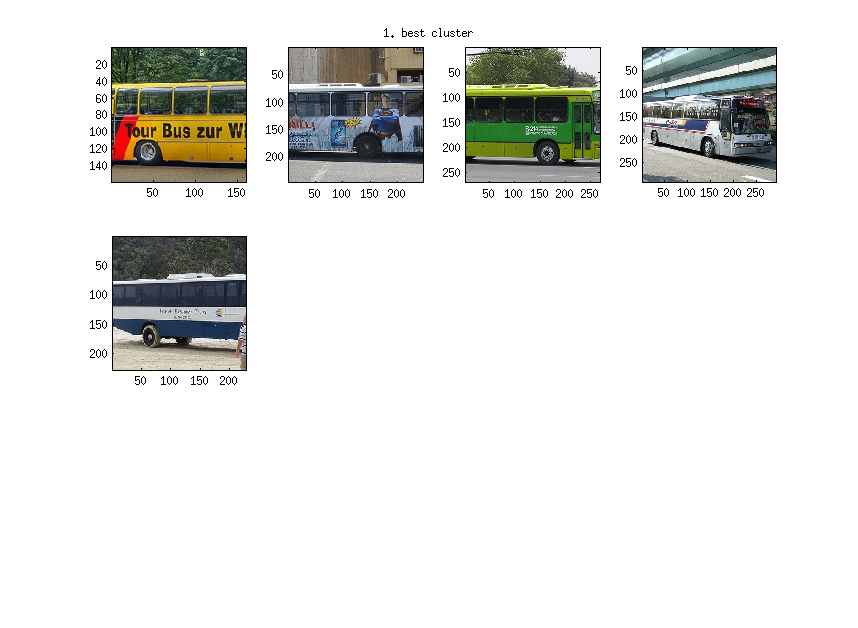
\includegraphics[height = 0.9\textheight]{pics/bus_best2_1.png}
\end{figure}
\end{frame}

\begin{frame}
\frametitle{Busses 2}
\begin{figure}
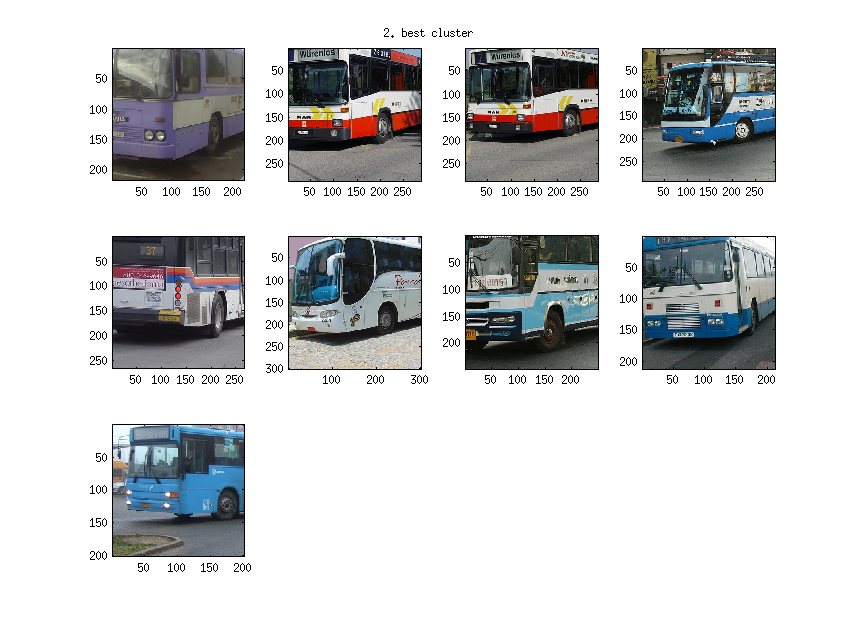
\includegraphics[width = 0.85\textwidth]{pics/bus_best2_2.png}
\end{figure}
\end{frame}

\begin{frame}
\frametitle{Busses 2}
\begin{figure}
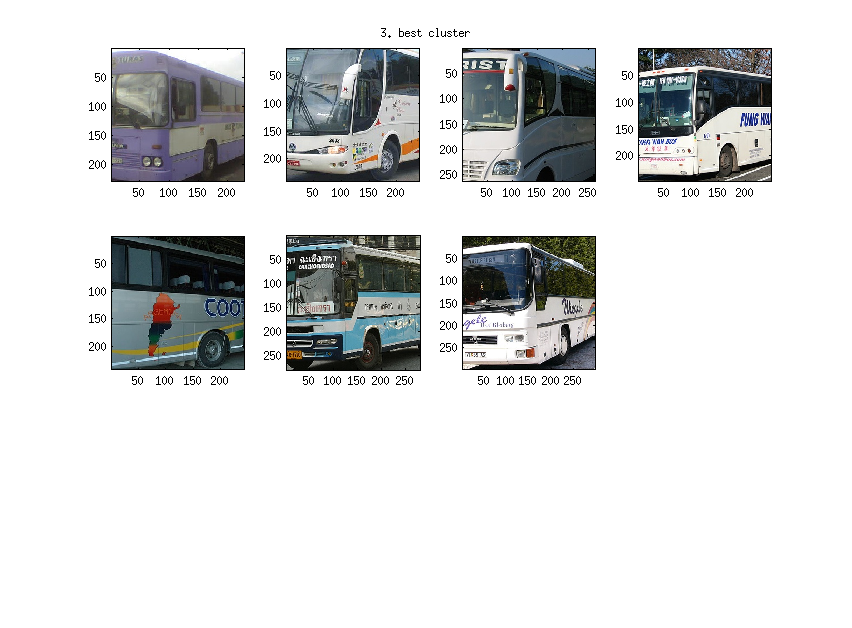
\includegraphics[width = 0.9\textwidth]{pics/bus_best2_3.png}
\end{figure}
\end{frame}

\begin{frame}
\frametitle{Busses 2}
\begin{figure}
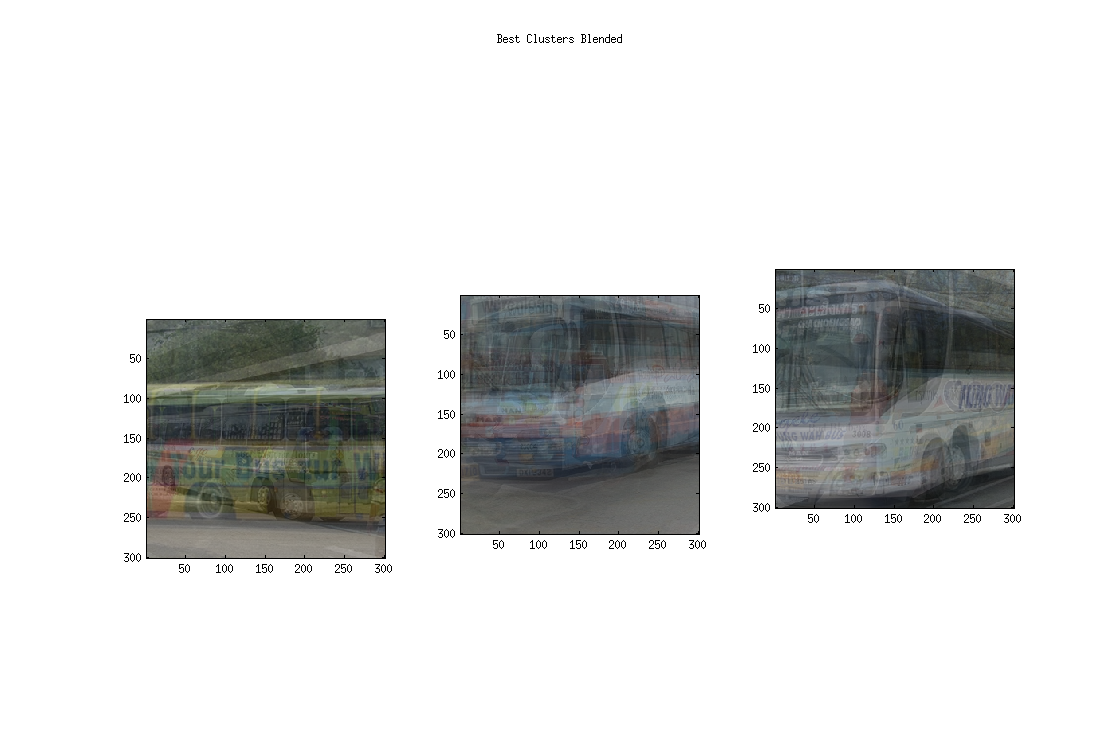
\includegraphics[width = 0.9\textwidth]{pics/bus_best2_blend.png}
\end{figure}
\end{frame}


\begin{frame}
\frametitle{Horses}
\begin{figure}
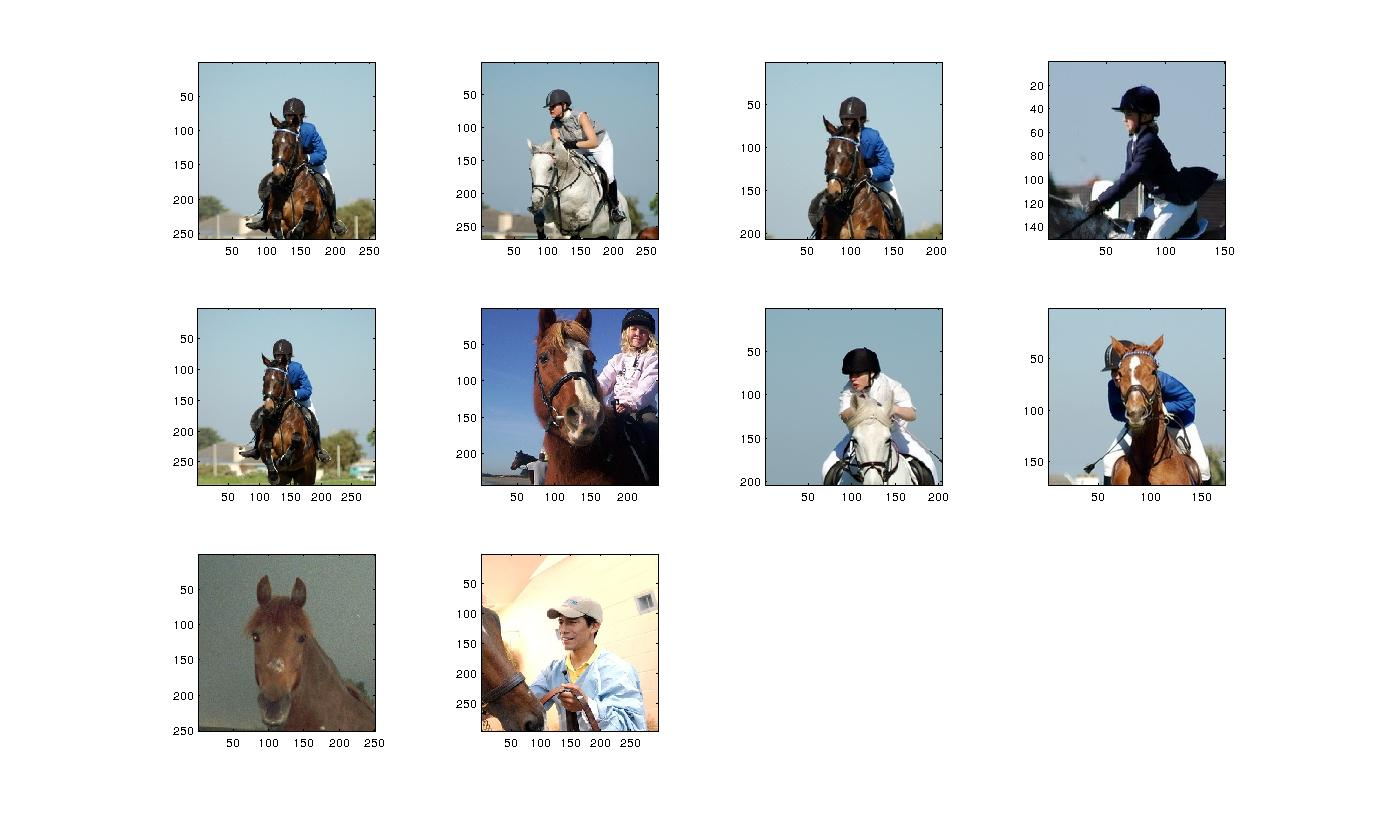
\includegraphics[width = 0.85\textwidth]{pics/horse_rider.jpg}
\end{figure}
\end{frame}

\begin{frame}
\frametitle{Horses}
\begin{figure}
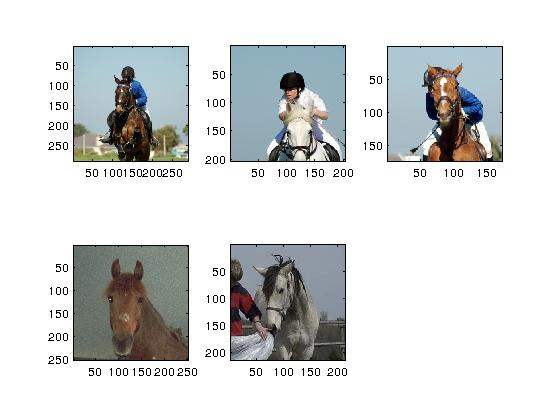
\includegraphics[width = 0.80\textwidth]{pics/pferdegesichter.jpg}
\end{figure}
\end{frame}

\begin{frame}
\frametitle{Horses}
\begin{figure}
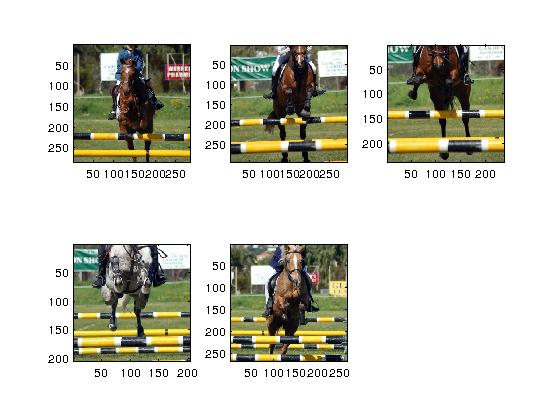
\includegraphics[width = 0.80\textwidth]{pics/jumping_horse.jpg}
\end{figure}
\end{frame}

\begin{frame}
\frametitle{Horses}
\begin{figure}
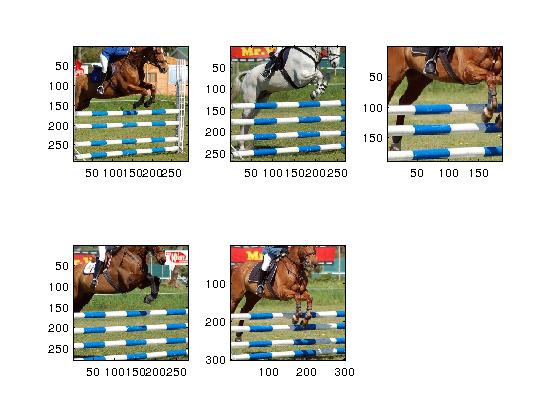
\includegraphics[width = 0.80\textwidth]{pics/jumping_horse_fence.jpg}
\end{figure}
\end{frame}



\begin{frame}
\frametitle{Bicycles}
\begin{figure}
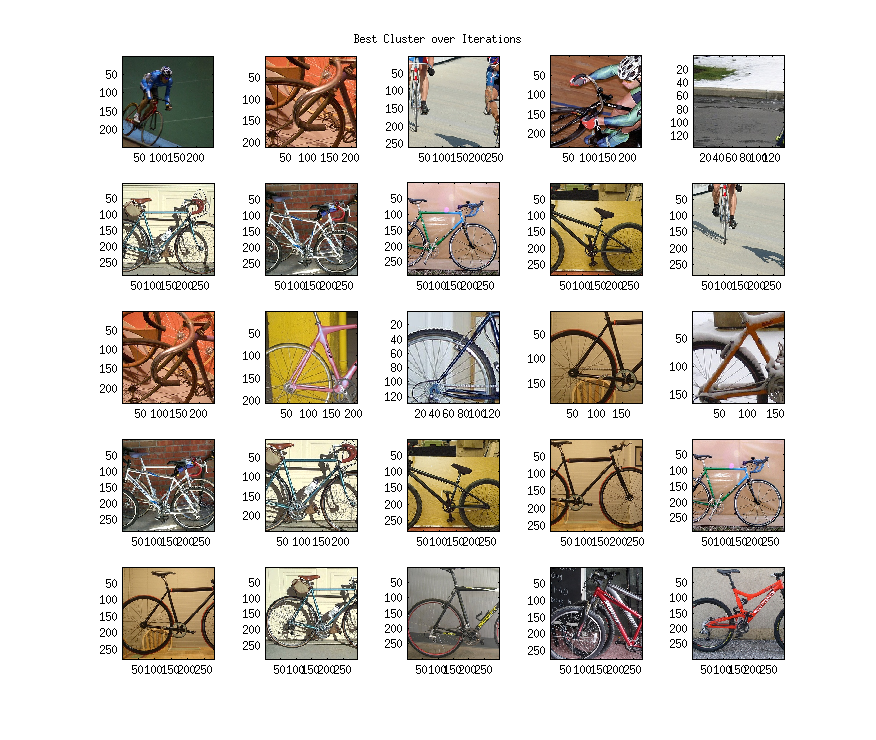
\includegraphics[width = 0.75\textwidth]{pics/bicycles_iter.png}
\end{figure}
\end{frame}




\subsection{MIT Indoor 67}
\begin{frame}
\frametitle{Airport}
\begin{figure}
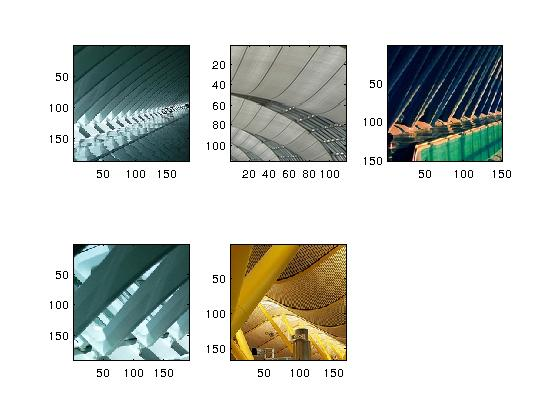
\includegraphics[width = 0.80\textwidth]{pics/airport_architecture.jpg}
\end{figure}
\end{frame}

\begin{frame}
\frametitle{Hairsalon}
\begin{figure}
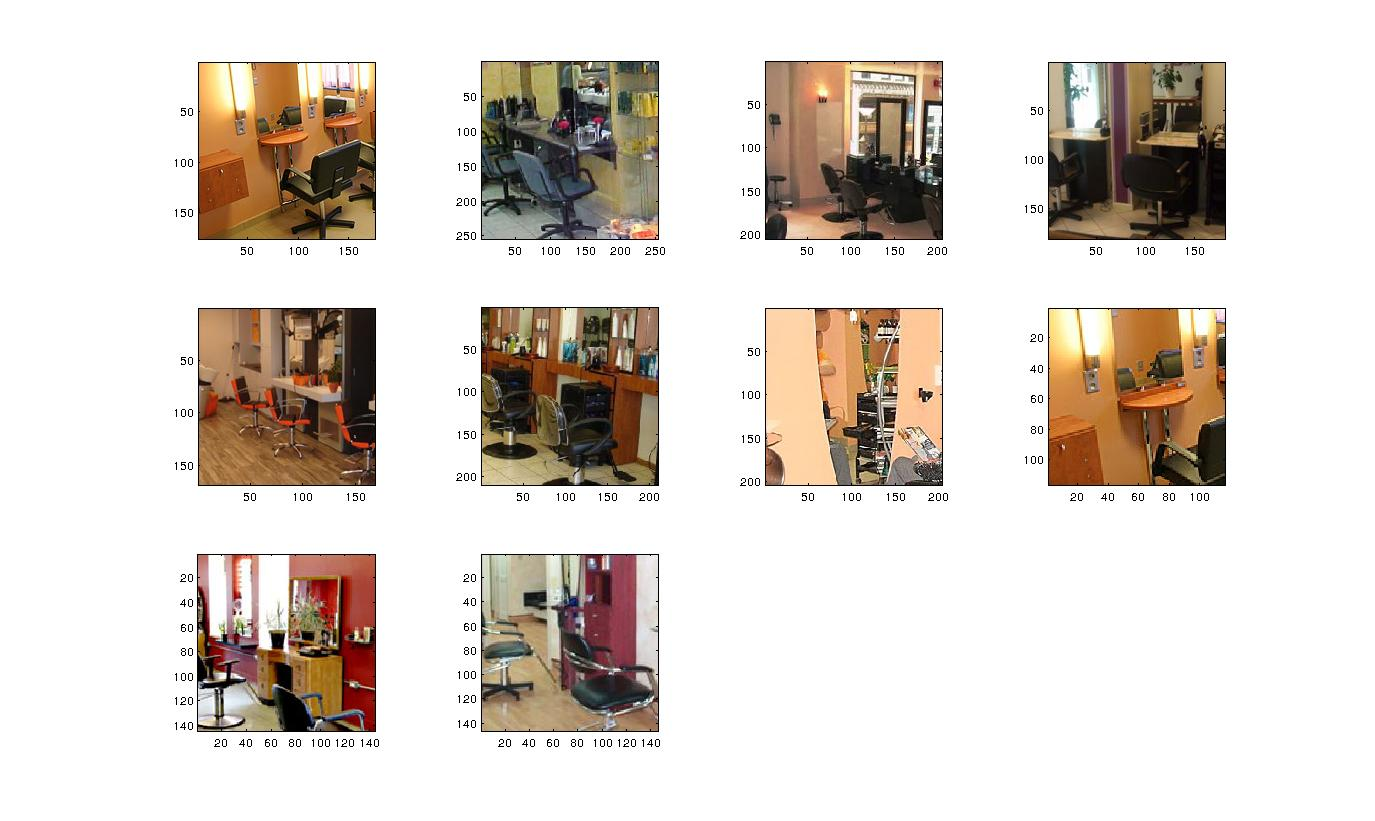
\includegraphics[width = 0.85\textwidth]{pics/hairsalon_chairs.jpg}
\end{figure}
\end{frame}



\section{Conclusions}
\subsection{}
\begin{frame}\frametitle{Results Singh et al. - Pascal VOC 07}
 \begin{figure}
  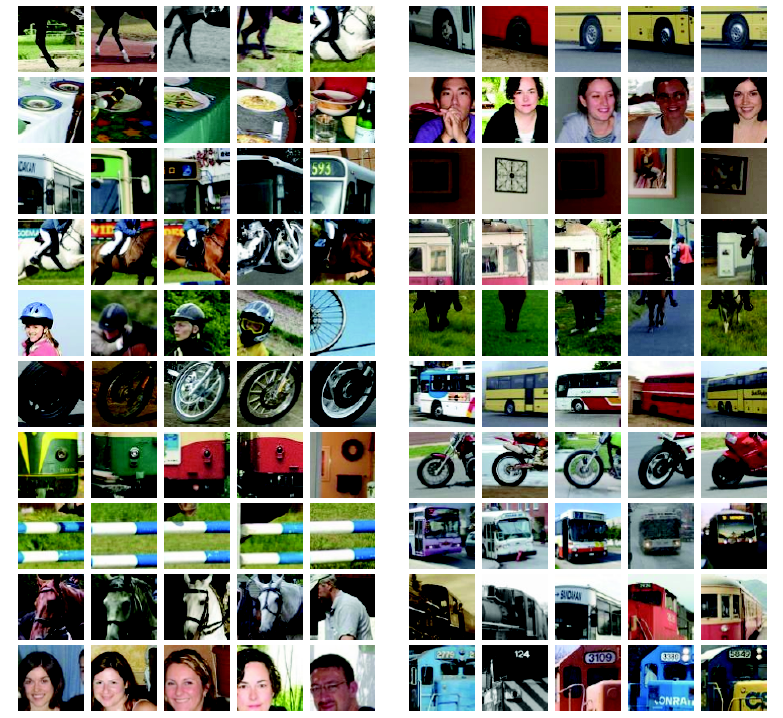
\includegraphics[scale = 0.26]{pics/results_singh_pascal.png}
  \end{figure}
\end{frame}

\begin{frame}\frametitle{Results Singh et al. - MIT Indoor 67}

\begin{centering}
 $\begin{array}{cc}
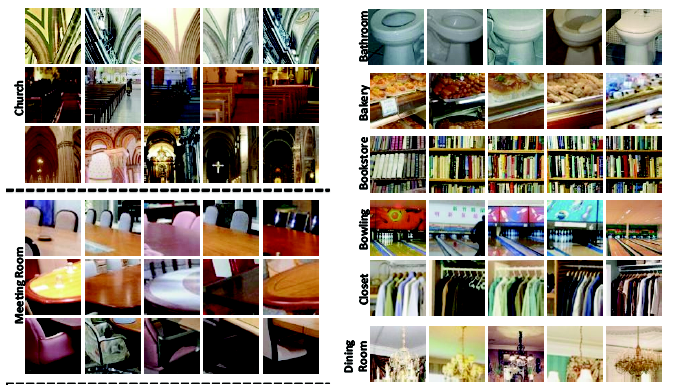
\includegraphics[scale = 0.22]{pics/results_singh_mit1.png} \hfill &
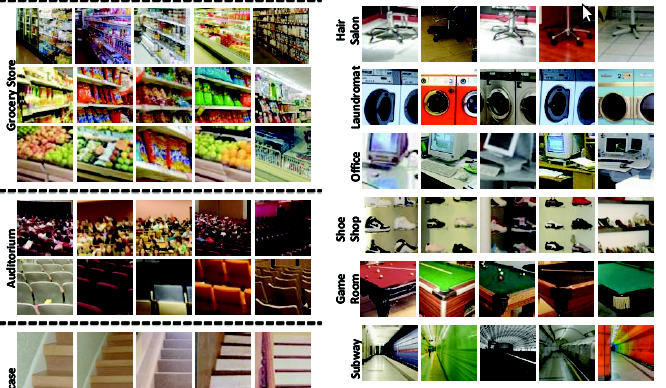
\includegraphics[scale = 0.22]{pics/results_singh_mit2.png}
\end{array}$
\end{centering}

\end{frame}

\begin{frame}
\begin{block}{Our thoughts}
 \begin{itemize}
  \item Promising method
  \item Computationally expensive
  \item ..but also reduced world set/discovery set yields passable results in most cases
 \end{itemize}
 \end{block}
\end{frame}

\begin{frame}
 \begin{block}{Le fin}
 \begin{centering}
   Thank you for your attention!
  \end{centering}
 \end{block}
\end{frame}



\end{document}